\documentclass[conference]{IEEEtran}

\usepackage{cite}
\usepackage{amsmath,amssymb,amsfonts}
\usepackage{graphicx}
\usepackage{textcomp}
\usepackage{booktabs}
\usepackage{multirow}
\usepackage{xcolor}
\usepackage{hyperref}
\usepackage{algorithm}
\usepackage{algorithmic}

\graphicspath{{figures/}}

\begin{document}

\title{Decentralized vs.\ Federated Learning for ICU Length-of-Stay Prediction: A Ring-Topology Gossip Approach on MIMIC-IV}

\author{
\IEEEauthorblockN{[Author Names]}
\IEEEauthorblockA{[Affiliation] \\
[City, Country] \\
[email]}
}

\maketitle

\begin{abstract}
Federated learning enables collaborative model training across hospitals without sharing patient data, but centralized aggregation introduces a single point of failure and communication bottleneck. We compare two communication topologies for ICU length-of-stay (LOS) prediction: Federated Averaging (FedAvg) with star topology and Decentralized Parallel SGD (D-PSGD) with ring gossip. Using MIMIC-IV, we simulate a 5-hospital federation with clinically motivated non-IID partitioning based on ICU care unit types. Our experiments quantify the accuracy--decentralization trade-off: FedAvg achieves [X.XX $\pm$ X.XX] MAE while D-PSGD reaches [X.XX $\pm$ X.XX] MAE with [XX\%] higher communication cost but no central server dependency. We analyze per-hospital fairness, convergence speed, and the effect of local training epochs on both topologies. To our knowledge, this is the first comparison of FedAvg and D-PSGD for ICU LOS prediction on MIMIC-IV with a care-unit-based hospital partition.
\end{abstract}

\begin{IEEEkeywords}
Federated learning, decentralized learning, gossip protocols, ICU length-of-stay prediction, MIMIC-IV
\end{IEEEkeywords}


% ============================================================
\section{Introduction}
\label{sec:introduction}

Accurate prediction of ICU length of stay (LOS) supports resource allocation, discharge planning, and cost estimation~\cite{}. Machine learning models trained on electronic health records (EHR) have shown promise for LOS prediction, but training on multi-site data raises privacy concerns under regulations such as HIPAA and GDPR.

Federated learning (FL) addresses this by training a shared model without centralizing patient data~\cite{mcmahan2017communication}. The dominant FL paradigm, Federated Averaging (FedAvg), uses a star topology where a central server aggregates model updates. While effective, this design introduces (i) a single point of failure, (ii) a communication bottleneck at the server, and (iii) trust assumptions about the aggregator.

Fully decentralized alternatives such as Decentralized Parallel SGD (D-PSGD)~\cite{lian2017can} eliminate the central server entirely. Each node communicates only with its neighbors in a predefined topology (e.g., ring), using gossip-based model averaging. This raises a key question:

\textbf{Research Question:} How does the choice of communication topology---centralized FedAvg (star) vs.\ decentralized D-PSGD (ring)---affect convergence and accuracy for ICU length-of-stay prediction across non-IID hospital data?

\textbf{Contributions:}
\begin{enumerate}
    \item First comparison of FedAvg vs.\ D-PSGD for ICU LOS prediction on MIMIC-IV.
    \item Clinically motivated non-IID partition: 5 simulated hospitals based on ICU care unit types, creating realistic data heterogeneity.
    \item Quantification of the accuracy cost of full decentralization (ring gossip vs.\ central server).
    \item Fairness analysis: do smaller or specialized hospitals benefit differently from each topology?
\end{enumerate}


% ============================================================
\section{Related Work}
\label{sec:related}

\subsection{ICU Length-of-Stay Prediction}

% TODO: Fill in related work on LOS prediction models (APACHE, SAPS, ML approaches)

\subsection{Federated Learning in Healthcare}

% TODO: Fill in FL in healthcare (FedAvg applications, privacy-preserving EHR)

\subsection{Decentralized Learning}

% TODO: Fill in D-PSGD, gossip protocols, comparison with FL


% ============================================================
\section{Methods}
\label{sec:methods}

\subsection{Data and Cohort}

We use MIMIC-IV v2.2+~\cite{johnson2023mimic}, extracting ICU stays with LOS $> 0$ and $\leq 30$ days, excluding in-hospital deaths. Features include demographics, admission information, first-24-hour vital signs (heart rate, blood pressure, respiratory rate, SpO2, temperature), first-24-hour laboratory values (glucose, creatinine, BUN, hemoglobin, platelets, WBC, sodium, potassium, bicarbonate, lactate), complexity proxies (number of procedures and diagnoses), and DRG code as a categorical feature.

\subsection{5-Hospital Partition}

We partition stays by ICU care unit type to simulate 5 hospitals with clinically distinct patient populations (Table~\ref{tab:partition}).

\begin{table}[h]
\centering
\caption{5-hospital care-unit-based partition.}
\label{tab:partition}
\begin{tabular}{lll}
\toprule
Hospital & Care Units & Profile \\
\midrule
H1 (Medical) & MICU, MICU/SICU & General medical \\
H2 (Neuro) & Neuro Int., Neuro Step., Neuro SICU & Neurological \\
H3 (Surgical) & SICU & General surgical \\
H4 (Trauma) & TSICU & Trauma surgical \\
H5 (Cardiac) & CCU, CVICU & Cardiac care \\
\bottomrule
\end{tabular}
\end{table}

Unmatched care units default to H1. This creates realistic non-IID heterogeneity in label distributions and feature correlations across hospitals.

\subsection{Model Architecture}

All experiments use the same single-task MLP: 256 $\rightarrow$ 128 $\rightarrow$ 64 hidden units with BatchNorm, ReLU, and dropout (0.3) after each hidden layer, followed by a single linear output for LOS regression. We use Huber loss ($\delta = 5.0$) with Adam optimizer (lr = $10^{-3}$, weight decay = $10^{-4}$) and ReduceLROnPlateau scheduling.

\subsection{FedAvg (Star Topology)}

In FedAvg~\cite{mcmahan2017communication}, a central server broadcasts the global model to all $N = 5$ hospitals each round. Each hospital trains locally for $E$ epochs, then sends the updated model back. The server aggregates via weighted average (weights proportional to dataset size). Communication cost per round: $2N \times |\theta|$ parameters.

\subsection{D-PSGD (Ring Topology)}

In D-PSGD~\cite{lian2017can}, there is no central server. Hospitals are arranged in a ring: $H_1 \leftrightarrow H_2 \leftrightarrow H_3 \leftrightarrow H_4 \leftrightarrow H_5 \leftrightarrow H_1$. Each round, hospitals train locally for $E$ epochs, then exchange models with their 2 ring neighbors and average using Metropolis--Hastings mixing weights ($W_{ij} = 1/3$ for self and each neighbor). Communication cost per round: $2 \times 2 \times N \times |\theta|$ parameters.

\subsection{Baselines}

\begin{itemize}
    \item \textbf{Centralized MLP:} Same architecture trained on all pooled data (upper bound).
    \item \textbf{Centralized XGBoost:} XGBoost regressor on pooled data.
    \item \textbf{Local-only ($\times 5$):} Each hospital trains independently (lower bound).
\end{itemize}

\subsection{Evaluation}

\begin{itemize}
    \item \textbf{Metrics:} MAE, RMSE, R$^2$ on validation sets.
    \item \textbf{Convergence:} Rounds to reach 95\% of centralized MAE.
    \item \textbf{Communication cost:} Total model parameters exchanged.
    \item \textbf{Fairness:} Per-hospital MAE standard deviation.
    \item \textbf{Ablation:} Local epochs $E \in \{1, 3, 5\}$.
    \item \textbf{Reproducibility:} 5-seed mean $\pm$ std (seeds 42--46), 80/20 train/val split per hospital.
\end{itemize}


% ============================================================
\section{Results}
\label{sec:results}

\subsection{Main Comparison}

% TODO: Fill in actual numbers after full experiment run
\begin{table}[t]
\centering
\caption{Main comparison of all training strategies. MAE and RMSE in days; R$^2$ dimensionless; W-1d is \% of predictions within 1 day of true LOS. Mean $\pm$ std over 5 seeds.}
\label{tab:main}
\begin{tabular}{lcccc}
\toprule
Method & MAE $\downarrow$ & RMSE $\downarrow$ & R$^2$ $\uparrow$ & W-1d $\uparrow$ \\
\midrule
Centralized MLP & 1.717 � 0.014 & 3.215 � 0.186 & 0.277 � 0.098 & 0.540 � 0.004 \\
Centralized XGBoost & 1.747 � 0.011 & 2.943 � 0.018 & 0.397 � 0.009 & 0.501 � 0.005 \\
FedAvg (E=1) & 1.718 � 0.078 & 5.334 � 4.552 & -4.588 � 9.799 & 0.551 � 0.008 \\
FedAvg (E=3) & 1.676 � 0.013 & 3.059 � 0.140 & 0.315 � 0.062 & 0.557 � 0.004 \\
FedAvg (E=5) & 1.687 � 0.010 & 3.018 � 0.054 & 0.334 � 0.010 & 0.548 � 0.004 \\
D-PSGD (E=1) & 1.845 � 0.072 & 4.985 � 3.605 & -4.250 � 9.156 & 0.502 � 0.010 \\
D-PSGD (E=3) & 1.830 � 0.022 & 3.425 � 0.408 & 0.162 � 0.329 & 0.511 � 0.006 \\
D-PSGD (E=5) & 1.827 � 0.012 & 3.254 � 0.136 & 0.300 � 0.085 & 0.513 � 0.007 \\
Local-only (avg) & 1.753 � 0.267 & 3.327 � 0.557 & 0.260 � 0.245 & 0.550 � 0.065 \\
\bottomrule
\end{tabular}
\end{table}


Table~\ref{tab:main} presents the main results across all training strategies. The centralized MLP and XGBoost baselines represent the upper bound achievable with pooled data access.

\subsection{Convergence}

\begin{figure}[t]
\centering
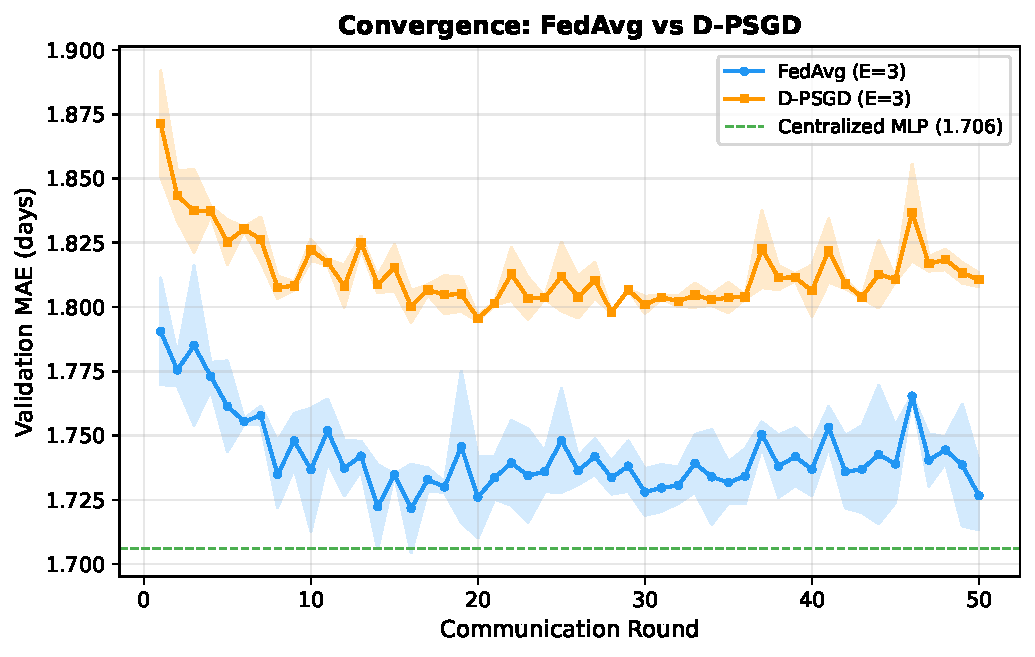
\includegraphics[width=\columnwidth]{fig2_convergence.pdf}
\caption{Convergence curves: validation MAE vs.\ communication rounds for FedAvg and D-PSGD ($E=3$). Shaded regions show $\pm 1$ std across 5 seeds. Dashed line indicates centralized MLP baseline.}
\label{fig:convergence}
\end{figure}

Figure~\ref{fig:convergence} shows the convergence behavior of FedAvg and D-PSGD over 50 rounds.

\subsection{Per-Hospital Performance}

\begin{table}[t]
\centering
\caption{Per-hospital MAE (days) for FedAvg, D-PSGD, and local-only (E=3, mean $\pm$ std over 5 seeds).}
\label{tab:per-hospital}
\begin{tabular}{lccc}
\toprule
Hospital & FedAvg & D-PSGD & Local-only \\
\midrule
H1 (Medical) & 1.673 $\pm$ 0.047 & 1.734 $\pm$ 0.054 & 1.610 $\pm$ 0.052 \\
H2 (Neuro) & 2.434 $\pm$ 0.078 & 2.296 $\pm$ 0.073 & 2.152 $\pm$ 0.049 \\
H3 (Surgical) & 1.820 $\pm$ 0.033 & 1.826 $\pm$ 0.016 & 1.761 $\pm$ 0.013 \\
H4 (Trauma) & 1.702 $\pm$ 0.023 & 1.693 $\pm$ 0.034 & 1.701 $\pm$ 0.090 \\
H5 (Cardiac) & 1.510 $\pm$ 0.021 & 1.504 $\pm$ 0.015 & 1.478 $\pm$ 0.026 \\
\bottomrule
\end{tabular}
\end{table}


\begin{figure}[t]
\centering
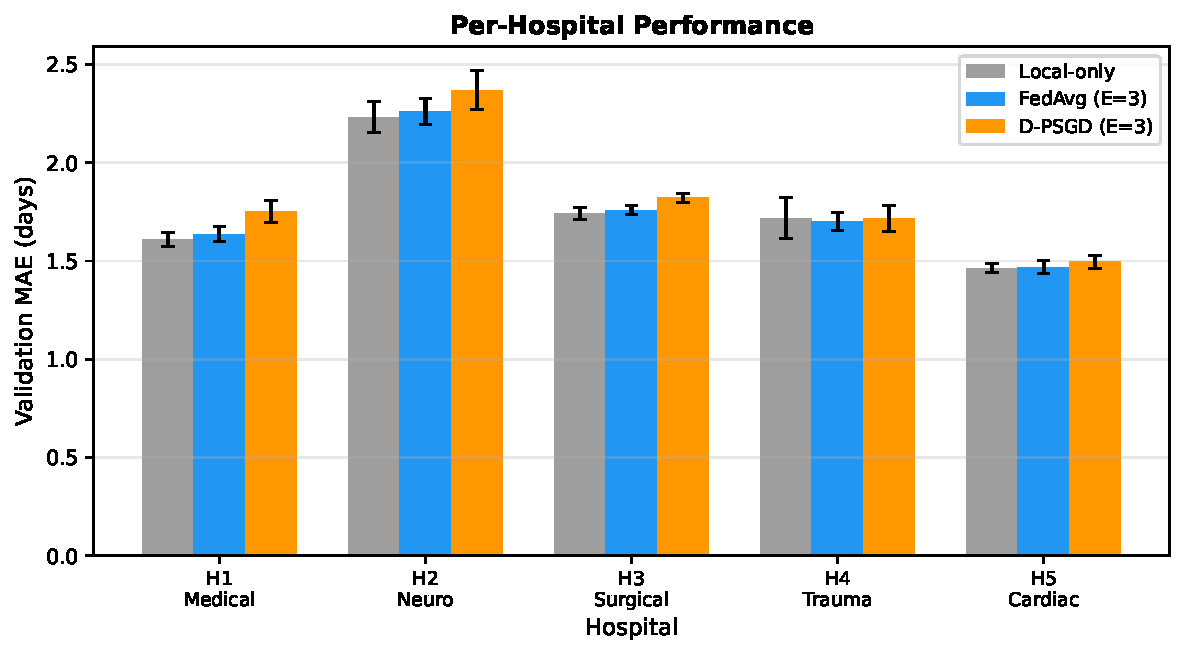
\includegraphics[width=\columnwidth]{fig3_per_hospital.pdf}
\caption{Per-hospital MAE for local-only, FedAvg, and D-PSGD ($E=3$). Error bars show $\pm 1$ std across 5 seeds.}
\label{fig:per-hospital}
\end{figure}

Table~\ref{tab:per-hospital} and Figure~\ref{fig:per-hospital} break down performance by hospital.

\subsection{Ablation: Local Epochs}

\begin{figure}[t]
\centering
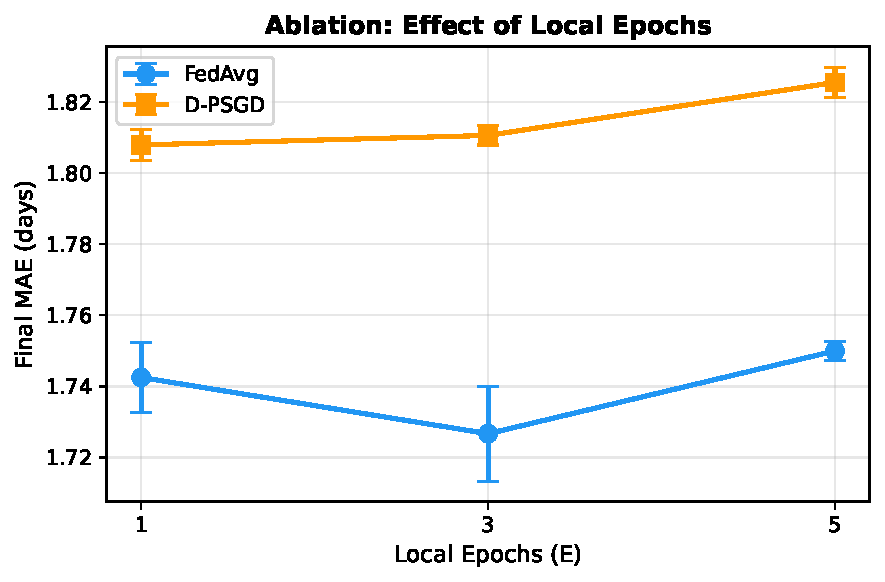
\includegraphics[width=\columnwidth]{fig4_ablation.pdf}
\caption{Effect of local epochs ($E = 1, 3, 5$) on final MAE for FedAvg and D-PSGD. Error bars show $\pm 1$ std across 5 seeds.}
\label{fig:ablation}
\end{figure}

\subsection{Communication Cost}

\begin{figure}[t]
\centering
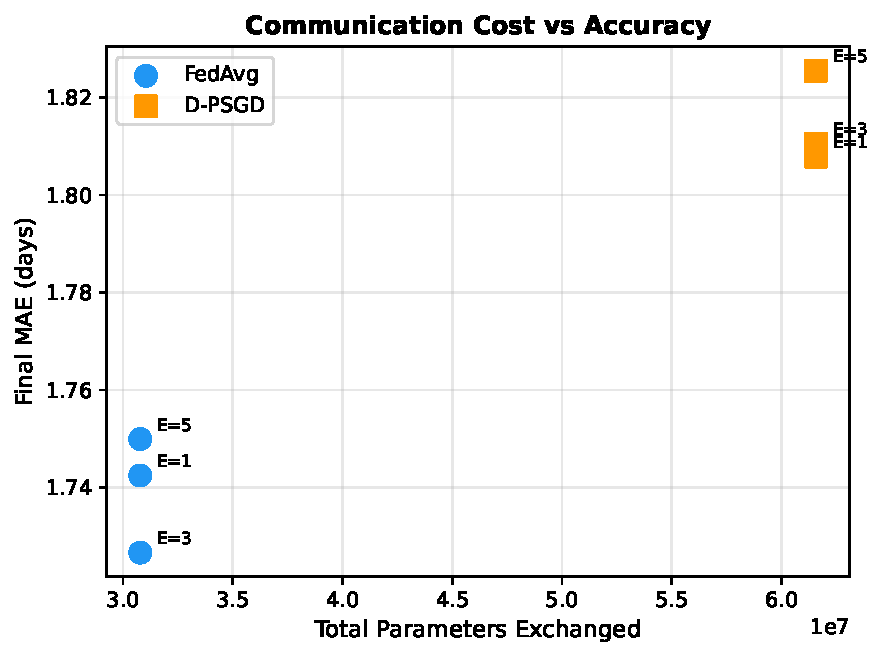
\includegraphics[width=\columnwidth]{fig5_cost_accuracy.pdf}
\caption{Communication cost (total parameters exchanged) vs.\ final MAE for FedAvg and D-PSGD at different local epoch settings.}
\label{fig:cost}
\end{figure}


% ============================================================
\section{Discussion}
\label{sec:discussion}

% TODO: Interpret results, discuss trade-offs, fairness implications

\subsection{Accuracy--Decentralization Trade-off}

% TODO: Discuss how much accuracy D-PSGD sacrifices vs. the architectural benefits

\subsection{Fairness Across Hospitals}

% TODO: Discuss which hospitals benefit from which topology

\subsection{Limitations}

\begin{itemize}
    \item Global StandardScaler fitted on all data, simulating a pre-federation calibration step.
    \item No differential privacy (DP-SGD)---future work.
    \item Simulated federation (single machine), not distributed deployment.
    \item Validation set used for both early stopping and final evaluation.
    \item 5-hospital simulation may not capture dynamics of larger federations.
\end{itemize}


% ============================================================
\section{Conclusion}
\label{sec:conclusion}

% TODO: Summarize findings and contributions

We presented the first comparison of FedAvg (star) and D-PSGD (ring gossip) for ICU length-of-stay prediction on MIMIC-IV with clinically motivated non-IID partitioning.

% Future work: DP-SGD, larger federations, more complex topologies, multi-task learning.


% ============================================================
\bibliographystyle{IEEEtran}
\bibliography{references}

\end{document}
